\documentclass[conference]{IEEEtran}
\usepackage[cmex10]{amsmath}
\usepackage{xcolor}
\usepackage{graphicx}
\hyphenation{op-tical net-works semi-conduc-tor}

\begin{document}
\title{Week 3 Report\\ECE 432 Microwave Circuit Design II}
\author{\IEEEauthorblockN{Jackson Pugh}
\IEEEauthorblockA{Portland State University\\
Portland, OR 97207\\
Email: japugh@pdx.edu}
\and
\IEEEauthorblockN{Michael Woodruff}
\IEEEauthorblockA{Portland State University\\
Portland, OR 97207\\
Email: michael.woodruff@pdx.edu}}
\maketitle
\IEEEpeerreviewmaketitle
\section{Introduction}

\section{Questions \& Answers}
1. Read in one of the S-parameters datafiles for SAV-541+ and plot the frequency dependence of S21, S11 and K (use dB plot). In which region is it unconditionally stable: i.e. where is K$>$1 and $|\Delta|<$1, or $\mu$ $>$ 1? (one of criteria is sufficient)\\\\
\textcolor{red}{Looking at Figure~\ref{fig:stable}, the region where $\mu>1$ is: 3.76 - 10.35 GHz.}

\begin{figure}[!h]
\centering
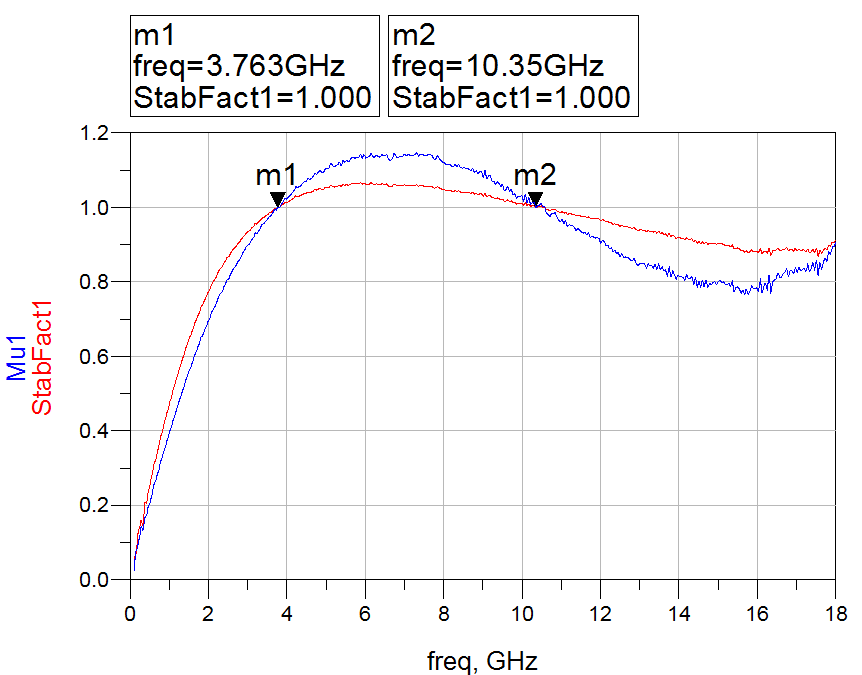
\includegraphics[scale=0.35]{pic/1stable.png}
\caption{Plot of $\mu$ and StabFact (K) from S2P manufacturer data.  Transistor stability region is inside the two markers.}
\label{fig:stable}
\end{figure}

2. Pick one frequency at which SAV-451+\footnote{SAV-541+} is unconditionally stable and design input and output matching for maximum transducer gain (simultaneous conjugate match). Construct the circuit in ADS and verify your "hand" calculation. Plot the values of gain and of $|$S21$|^2$ for the device alone around some (narrow) frequency range around the center frequency. Comment on your results.\\\\
\textcolor{red}{Choose 6 GHz:\\\\
Looking at Table~\ref{sparam} which was provided from the manufacturer S2P file, lists the S-Parameters at approximately 6 GHz.  These were used to calculate $\Gamma_{MS}$ and  $\Gamma_{ML}$, which are listed in Table~\ref{refco}\footnote{ADS also was able to calculate $\Gamma$ automatically}.  $\Gamma_{MS}$ and  $\Gamma_{ML}$  were plotted on the Smith Chart and then were matched using an open-stub matching network.  Figure~\ref{fig:2} shows the values of gain and  $|$S21$|^2$ for the device.}

\begin{table}[!h]
    \caption {S-Parameters}
    \begin{tabular}{lll}
    S-Parameter & Magnitude & Angle ($^{\circ}$) \\ \hline
    S11         & 0.70750   & 93.98            \\
    S21         & 2.57416   & -6.897           \\
    S12         & 0.11976   & -5.765           \\
    S22         & 0.23939   & 105.25           \\
    \end{tabular}
\label{sparam}
\end{table}

\begin{table}[h!]
\caption {Reflection Coefficient}
    \begin{tabular}{lll}

    Reflection Coefficient & Magnitude & Angle ($^{\circ}$) \\ \hline
    $\Gamma_{MS}$          & 0.834     & 97.80              \\
    $\Gamma_{ML}$          & 0.468     & 135.13             \\
    \end{tabular}
\label{refco}
\end{table}

\begin{figure}[!h]
\centering
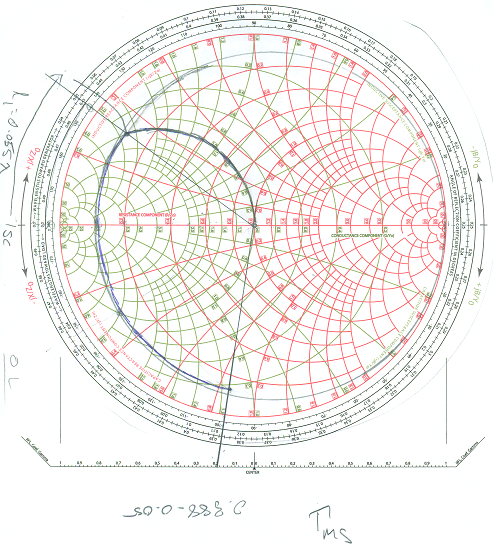
\includegraphics[scale=0.5]{pic/smith1.png}
\caption{Input reflection coefficient Smith Chart.  Matching network using an open-circuit stub is overlaid the Smith Chart.}
\label{fig:smith1}
\end{figure}

\begin{figure}[!h]
\centering
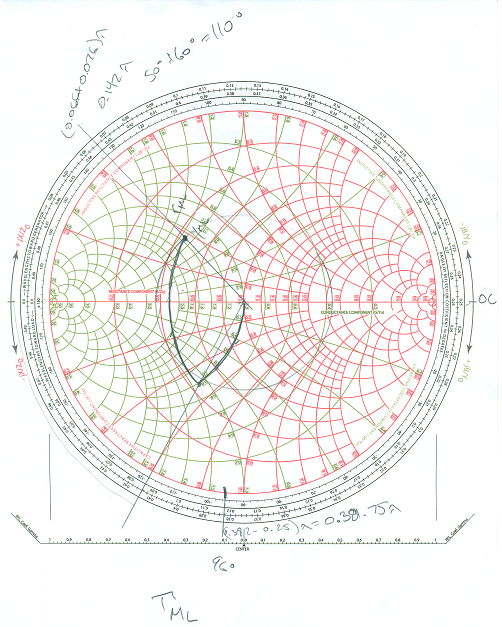
\includegraphics[scale=0.5]{pic/smith2.png}
\caption{Output reflection coefficient Smith Chart.  Matching network using an open-circuit stub is overlaid the Smith Chart}
\label{fig:smith2}
\end{figure}

\begin{figure}[!h]
\centering
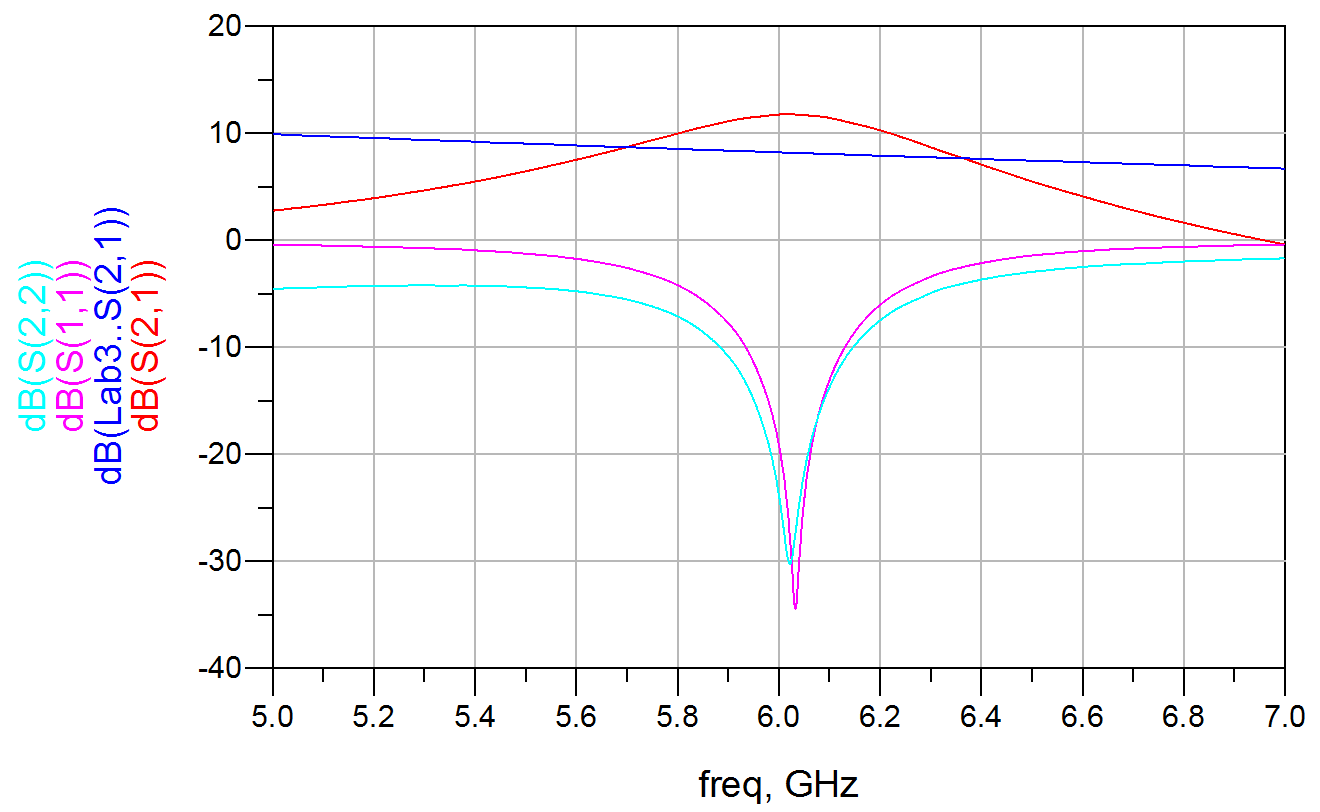
\includegraphics[scale=0.25]{pic/2.png}
\caption{Plot of S-Parameters after matching network is added.}
\label{fig:2}
\end{figure}

3. If you are restricted to values available from IEEE store, what are the values and what will happen to the match? Here is a list of what they are supposed to have:\\
a. Inductors: 1.3, 1.5, 1.8, 2.2, 2.7, 3.3, 3.9, 4.7, 5.6, 6.8, 8.2, 10, 12, 15, 18, 22 nH\\
b. Capacitors: 1, 1.3, 1.5, 1.8, 2.2, 2.7, 3.3, 3.9, 4.7, 5.6, 6.8, 8.2, 10, 12, 15, 18, 22, 33 pF\\\\
\textcolor{red}{If the comonents are not exact, then the conjugate matching network will not be as effective and there will be non-zero reflection at the ports}

4. Construct input and output stability circles at 2.4 GHz. Use these results to determine resistance to be placed in shunt on output that would make the device unconditionally stable. (a quick way to do this is in ADS will be demonstrated).\\\\
\textcolor{red}{Figure~\ref{fig:stabcircle} shows the input and output stability circles at 2.4 GHz.  A rough resistor shunt resistor value on the output to make the device unconditionally stable is 125 $\Omega$.  Optimizing this resistor in ADS gives a value near 120 $\Omega$.}
\begin{figure}[!h]
\centering
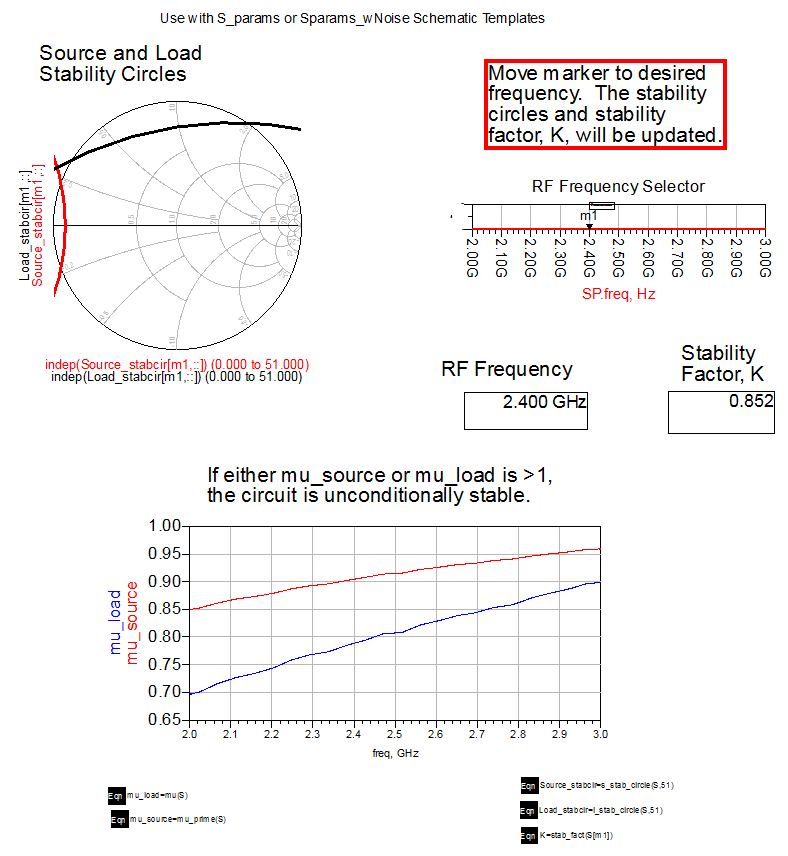
\includegraphics[scale=0.45]{pic/stabcircle.png}
\caption{Unoptimized stability circle at 2.4 GHz.  The circuit is potentially unstable.}
\label{fig:stabcircle}
\end{figure}

5. Implement this circuit in ADS and demonstrate that it is now unconditionally stable. If it is not, what would you do to fix that?\\\\
\textcolor{red}{Figure~\ref{fig:stabcircle-optimized} shows the result of adding a 120 $\Omega$ shunt resistor in the circuit.  The circuit is now unconditionally stable.}
\begin{figure}[!h]
\centering
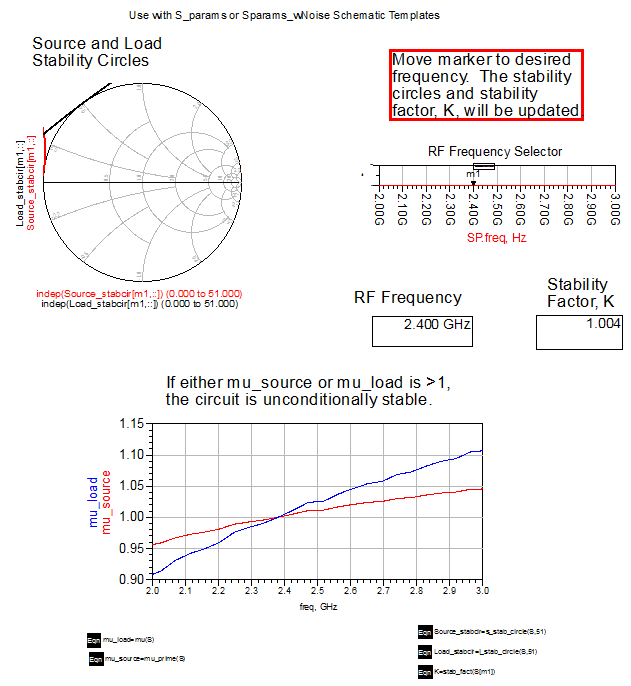
\includegraphics[scale=0.55]{pic/stabcircle-optimized.png}
\caption{Optimized stability circle at 2.4 GHz.  The circuit is unconditionally stable.}
\label{fig:stabcircle-optimized}
\end{figure}

6. Plot $|$S21$|$ and comment on the gain reduction compared to the original.\\\\
\textcolor{red}{Figure~\ref{fig:lastproblem} shows the gain and the original gain on the same plot.  The reduction is caused by adding the shunt resistor.}
\begin{figure}[!h]
\centering
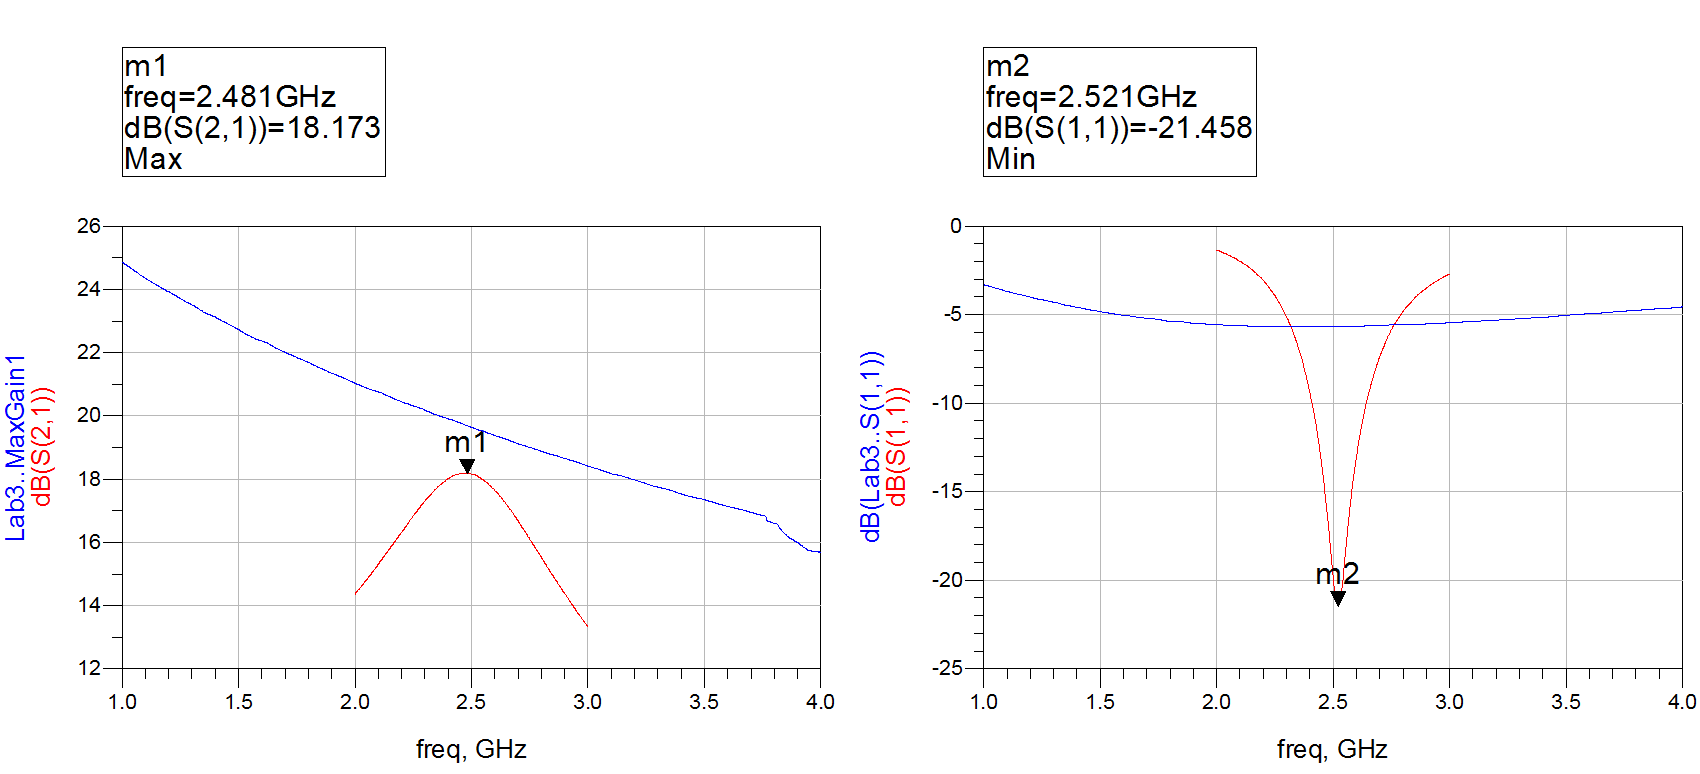
\includegraphics[scale=0.2]{pic/lastproblem.png}
\caption{Plot of original gain and the stabilized gain.  Note the reduction in the stabilized gain plot.}
\label{fig:lastproblem}
\end{figure}
\newpage
\section{Weekly Lessons}
\subsection{In-Class}
Stability Circles: The region of stability on the I/O stability circle is determined by the magnitude of $|$S11$|$ and $|$S22$|$.  If $|$S11$|$ or $|$S22$|$ $>$ 1, it is stable outside of the origin; if $|$S11$|$ or $|$S22$|$ $<$ 1 then it is stable inside the origin.  Anything outside of the stable region is considered potentially unstable.  In addition, to increase the stability region, a series/shunt resistor can be added to increase matching.  However, the downfall of this is a lower gain, due to a non-trivial voltage drop across the stabilizing resistor.
\subsection{Outside of Class}
Fundamentals of testing RF amplifiers and high-power devices with RF VNA\cite{agilent}: The Agilent webcast briefly reviewed S-Parameters and K (stability) factor.  Then the talk discussed the Agilent E5072A VNA features including a built-in calculator (equation editor) that can be used to calculate parameters such as K  and measuring high power output amplifiers using the direct receiver access (in addition to external components such as isolators/circulators).  It covered gain compression measurements by using a booster amplifier (in combination with power receiver leveling) to sample a high-power input\footnote{By high-power input this refers to an input signal that is higher than the analyzer can source} applied to a DUT.  Then it talked about measuring harmonic distortion (and intermodulation distortion) using Frequency-Offset Mode option which sweeps the input and output ports at different frequency ranges.  It then discussed different configurations to measure high-power input to a DUT and high-power output from a DUT.  Lastly, the webcast concluded the talk by explaining how to measuring specific applications such as RFID, SAW devices and antennas.
\begin{thebibliography}{1}
\bibitem{agilent}
Agilent Webcast: http://www.home.agilent.com/agilent/eventDetail.jspx?\\cc=US\&lc=eng\&ckey=2087011\&nid=-11143.0.00\&id=2087011
\end{thebibliography}
\end{document}